\begin{figure*}[]
	\vspace{-0.05in}
	\centering
	\subfigure[MNIST]{
		\begin{minipage}[t]{.25\linewidth}
			\centering
			%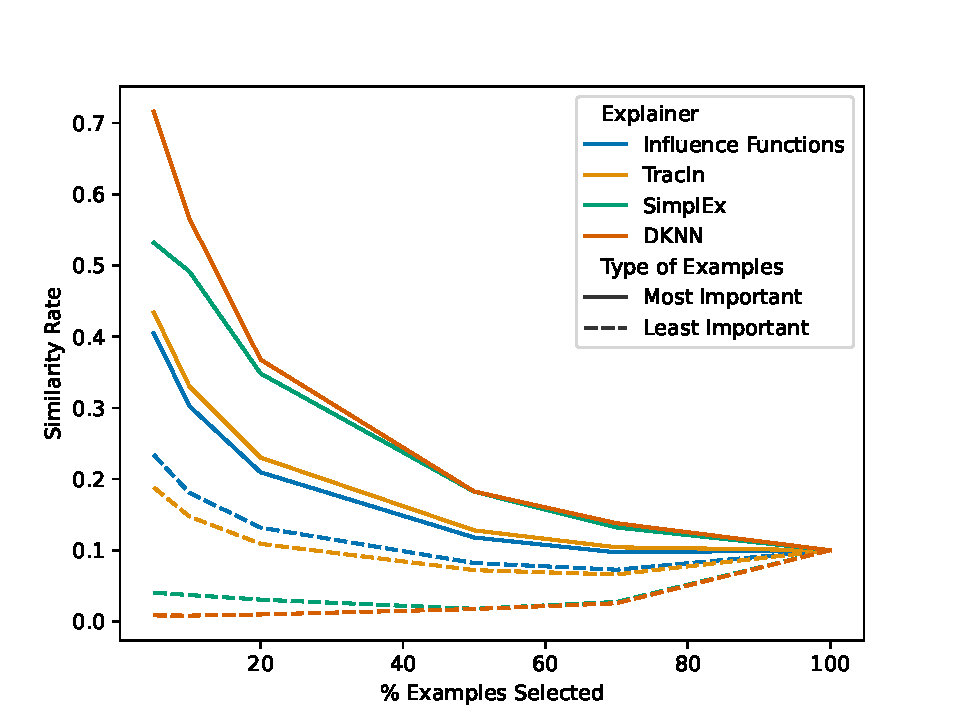
\includegraphics[width=1\linewidth]{img/og/mnist_similarity_rates}
            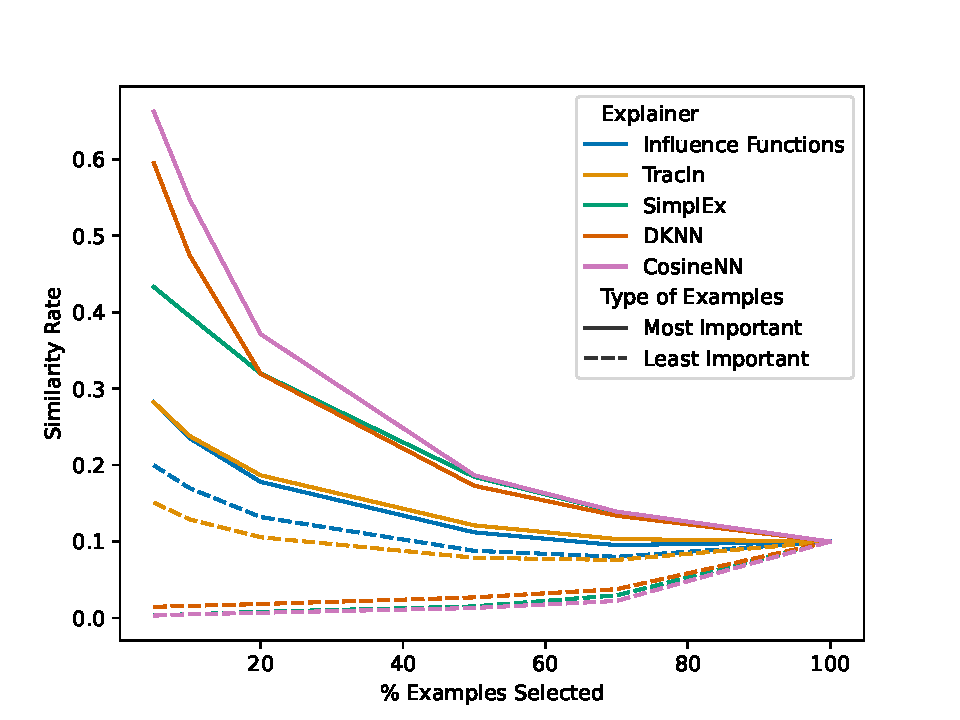
\includegraphics[width=1\linewidth]{img/extra/mnist_example_similarity_rates.pdf}
		\end{minipage}%
	}%
	\subfigure[ECG5000]{
		\begin{minipage}[t]{.25\linewidth}
			\centering
			%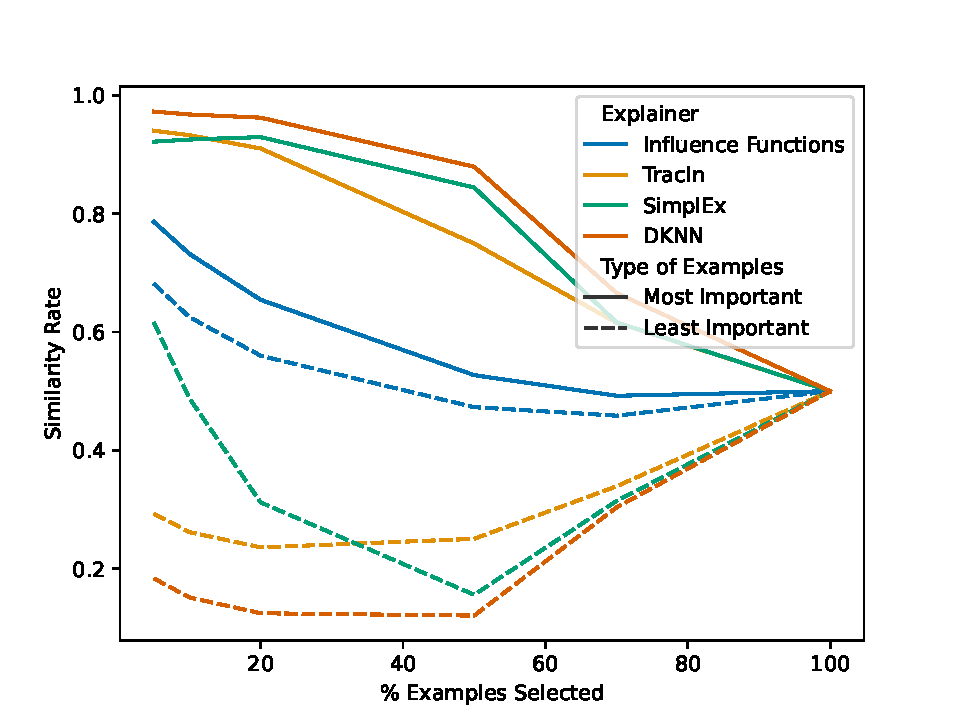
\includegraphics[width=1\linewidth]{img/og/ecg5000_similarity_rates}
            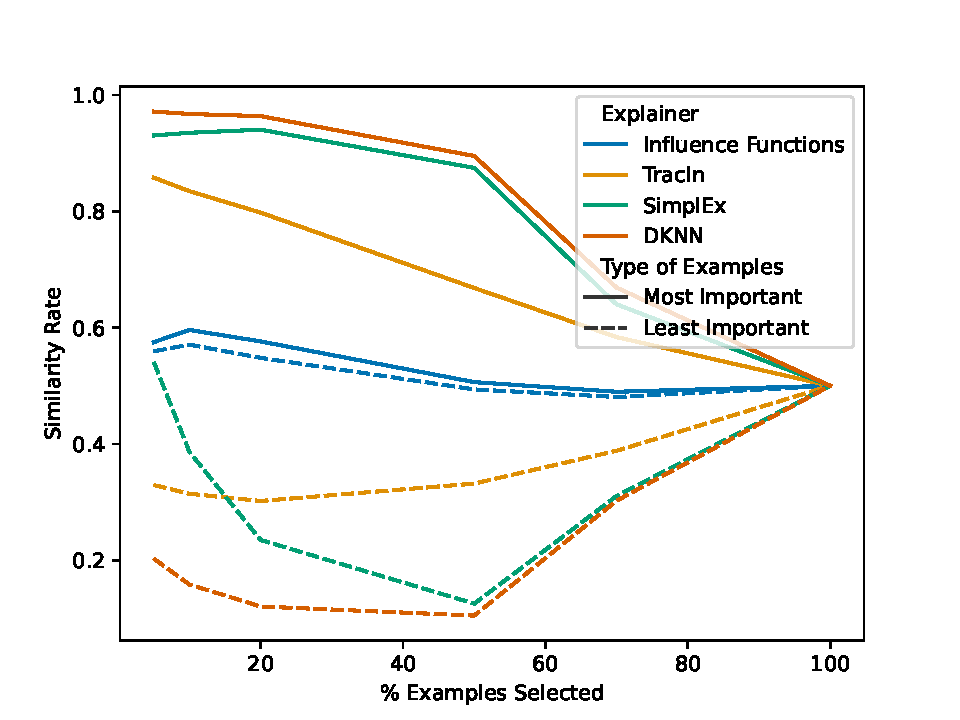
\includegraphics[width=1\linewidth]{img/rp/ecg5000_similarity_rates}
		\end{minipage}%
	}%
	\subfigure[CIFAR-10]{
		\begin{minipage}[t]{.25\linewidth}
			\centering
			%\includegraphics[width=1\linewidth]{img/og/cifar10_similarity_rates}
            \includegraphics[width=1\linewidth]{img/extra/cifar10_similarity_rates.pdf}
		\end{minipage}%
	}%
    \subfigure[CIFAR-100]{
		\begin{minipage}[t]{.25\linewidth}
			\centering
			%\includegraphics[width=1\linewidth]{img/og/cifar10_similarity_rates}
            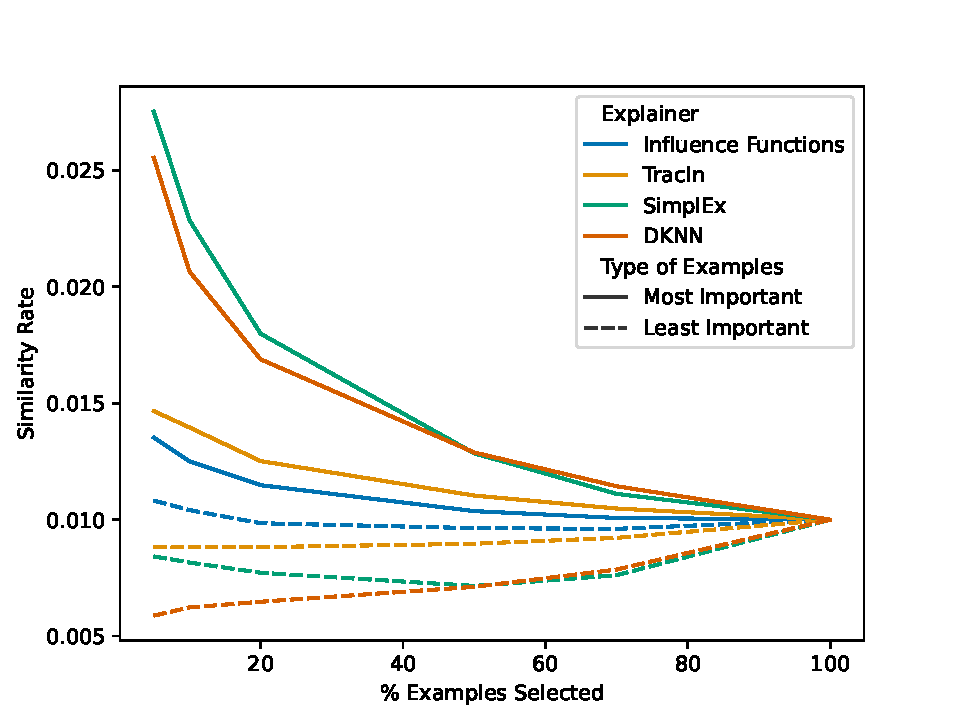
\includegraphics[width=1\linewidth]{img/extra/cifar100_similarity_rates.pdf}
		\end{minipage}%
	}%
	\vspace{-0.1in}
	\caption{Consistency check for label-free example importance. Each solid line shows how the similarity rate changes as we calculate it over some percentage of the highest-ranked training examples, for each choice of label-free example importance metric. The dotted lines show what happens if we start with the bottom-ranked samples instead.}
	\label{fig:cons_examples}
	\vspace{-0.1in}
\end{figure*}